\documentclass[12pt]{article}
\usepackage{graphicx}
\usepackage{amsmath}
\usepackage[margin=1in]{geometry}
\begin{document}
\section*{Worksheet B}
\begin{enumerate}
\item Calculate the rate of change from the graph below.

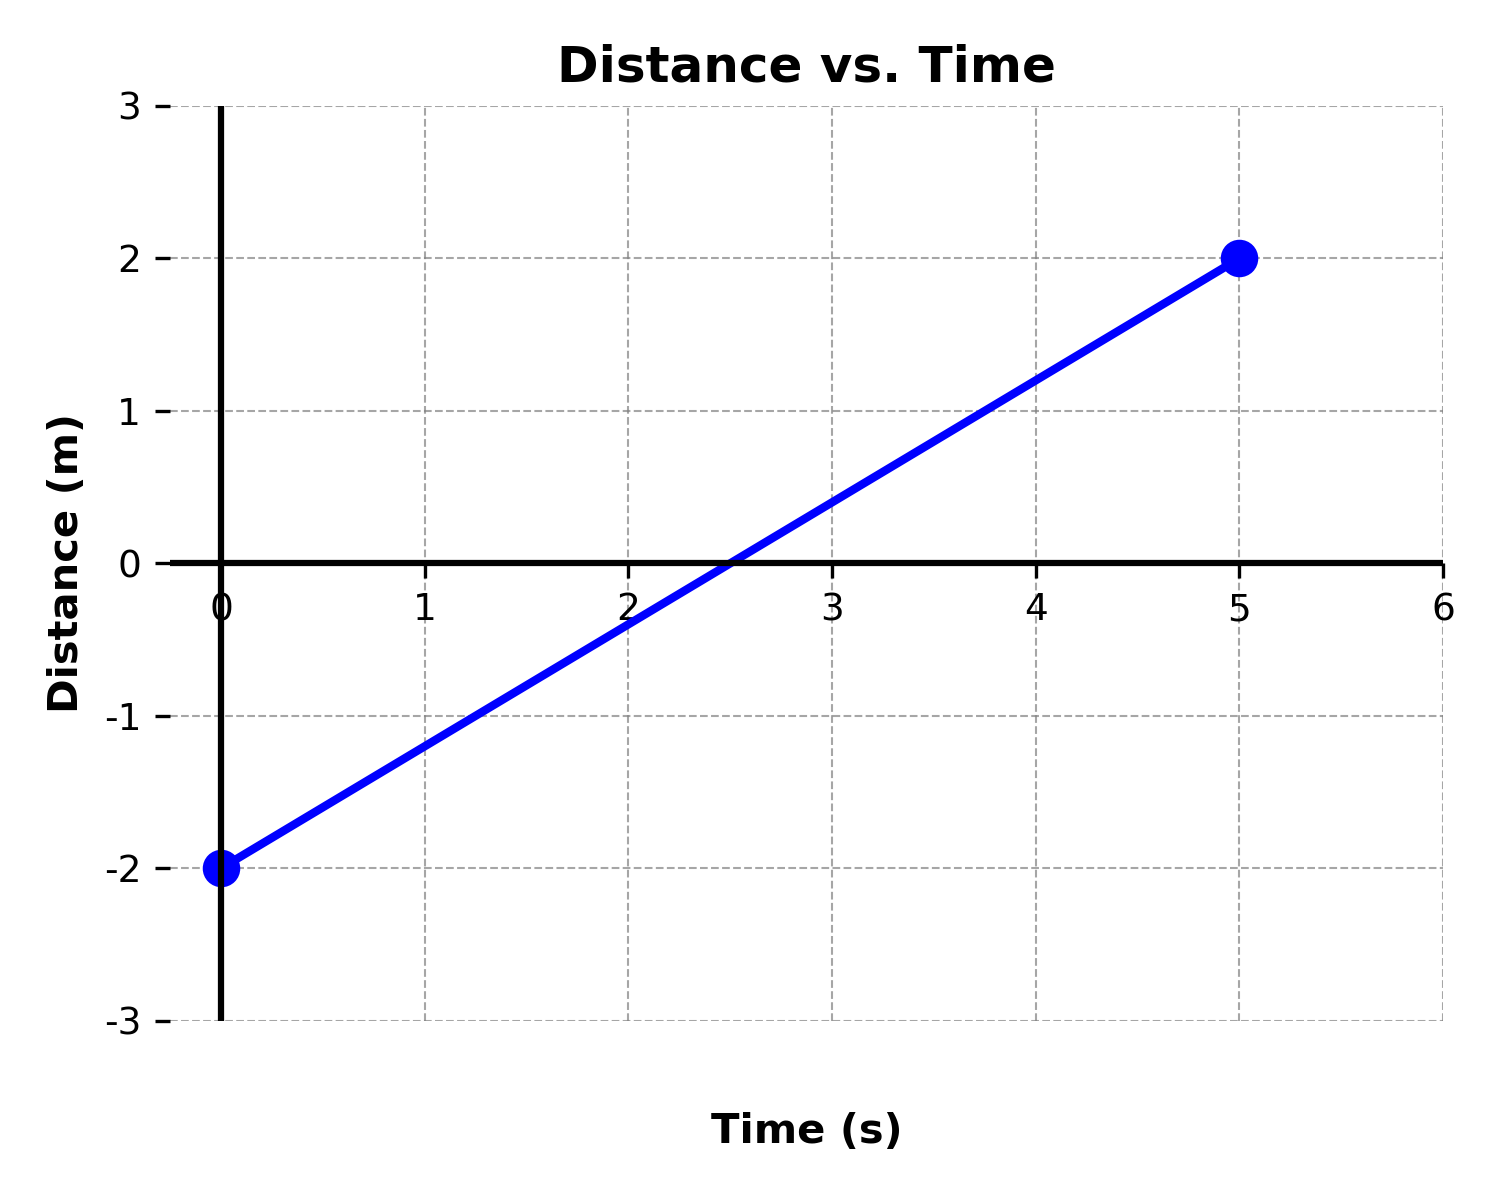
\includegraphics[width=0.6\textwidth]{B_problem_1.png}


\vspace{2cm}  % Add space for students to work
\item Calculate the rate of change from the graph below.

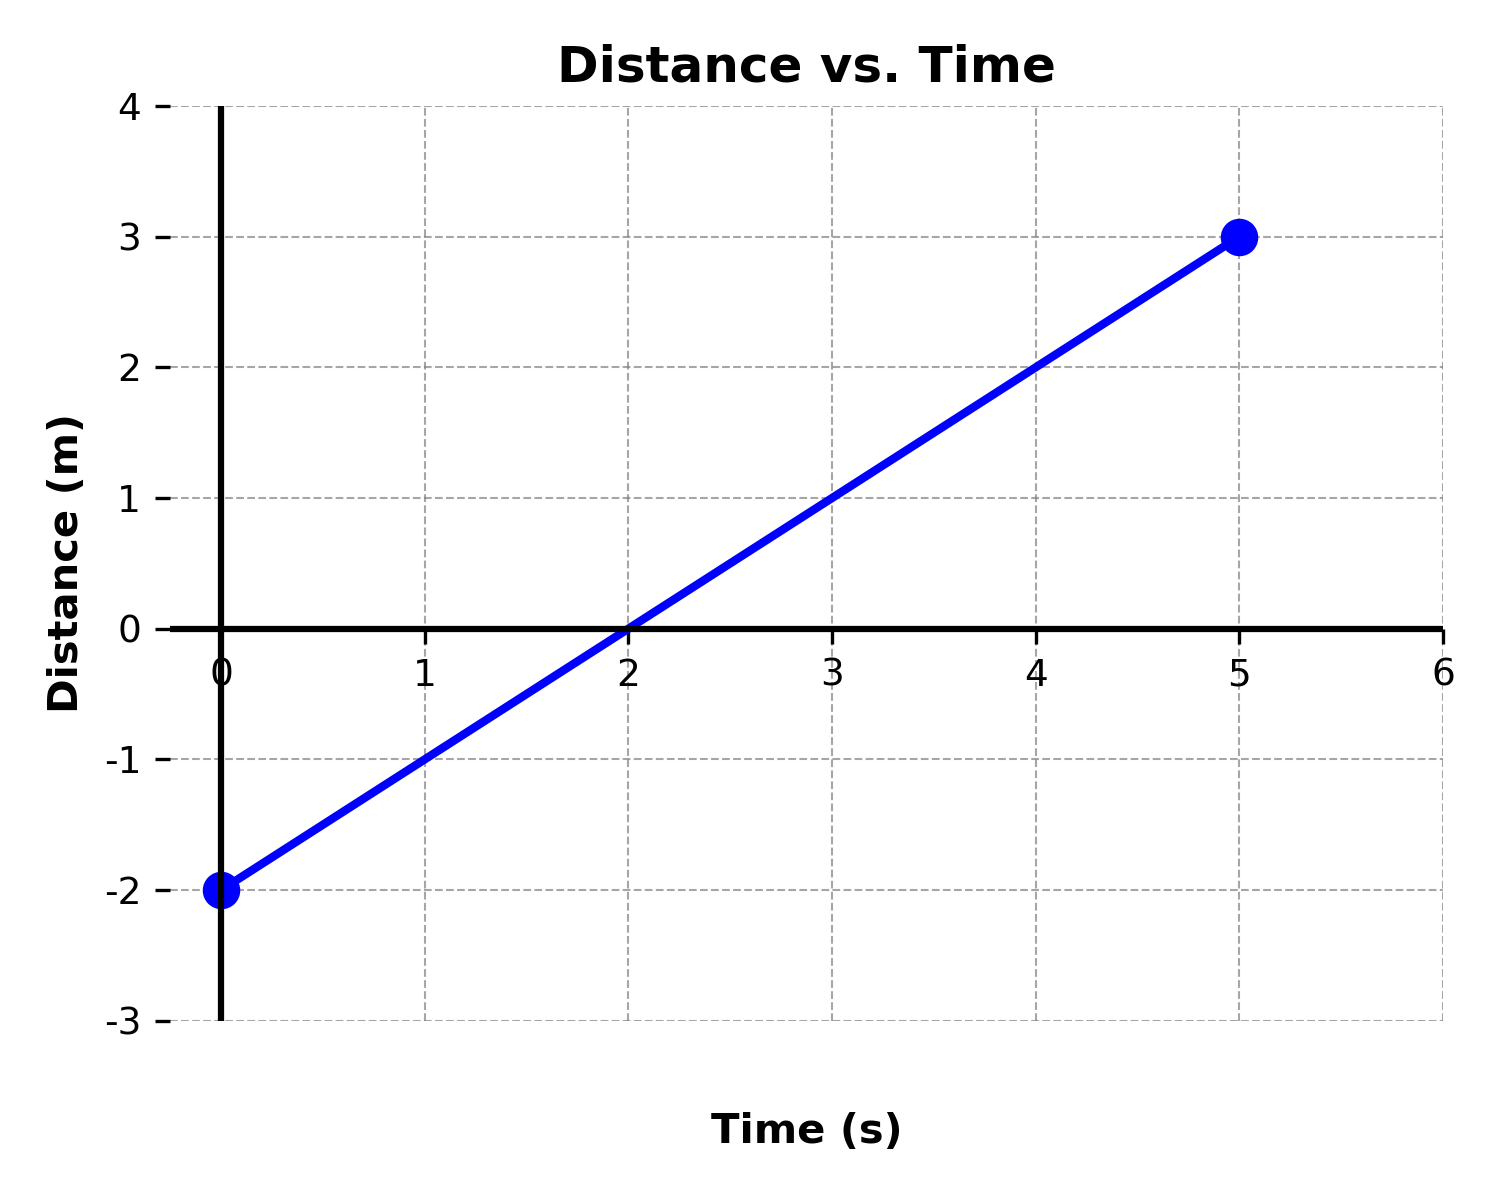
\includegraphics[width=0.6\textwidth]{B_problem_2.png}


\vspace{2cm}  % Add space for students to work
\item Calculate the rate of change from the graph below.

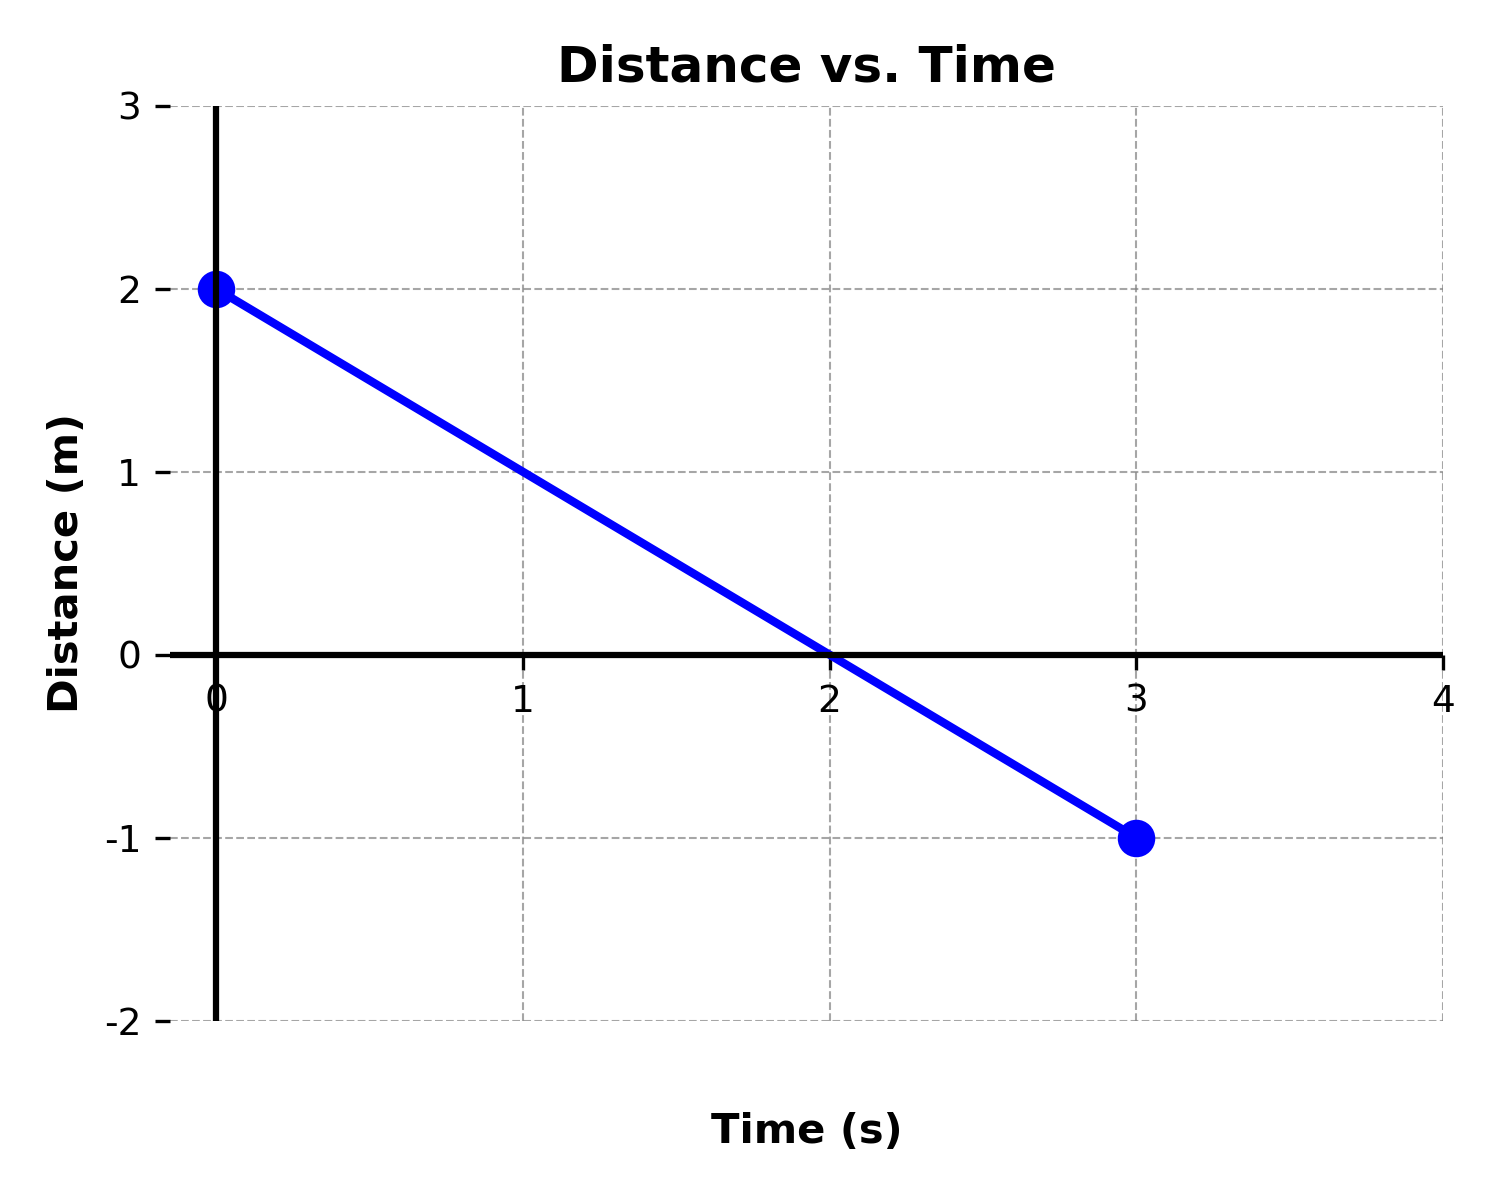
\includegraphics[width=0.6\textwidth]{B_problem_3.png}


\vspace{2cm}  % Add space for students to work
\item Calculate the rate of change from the graph below.

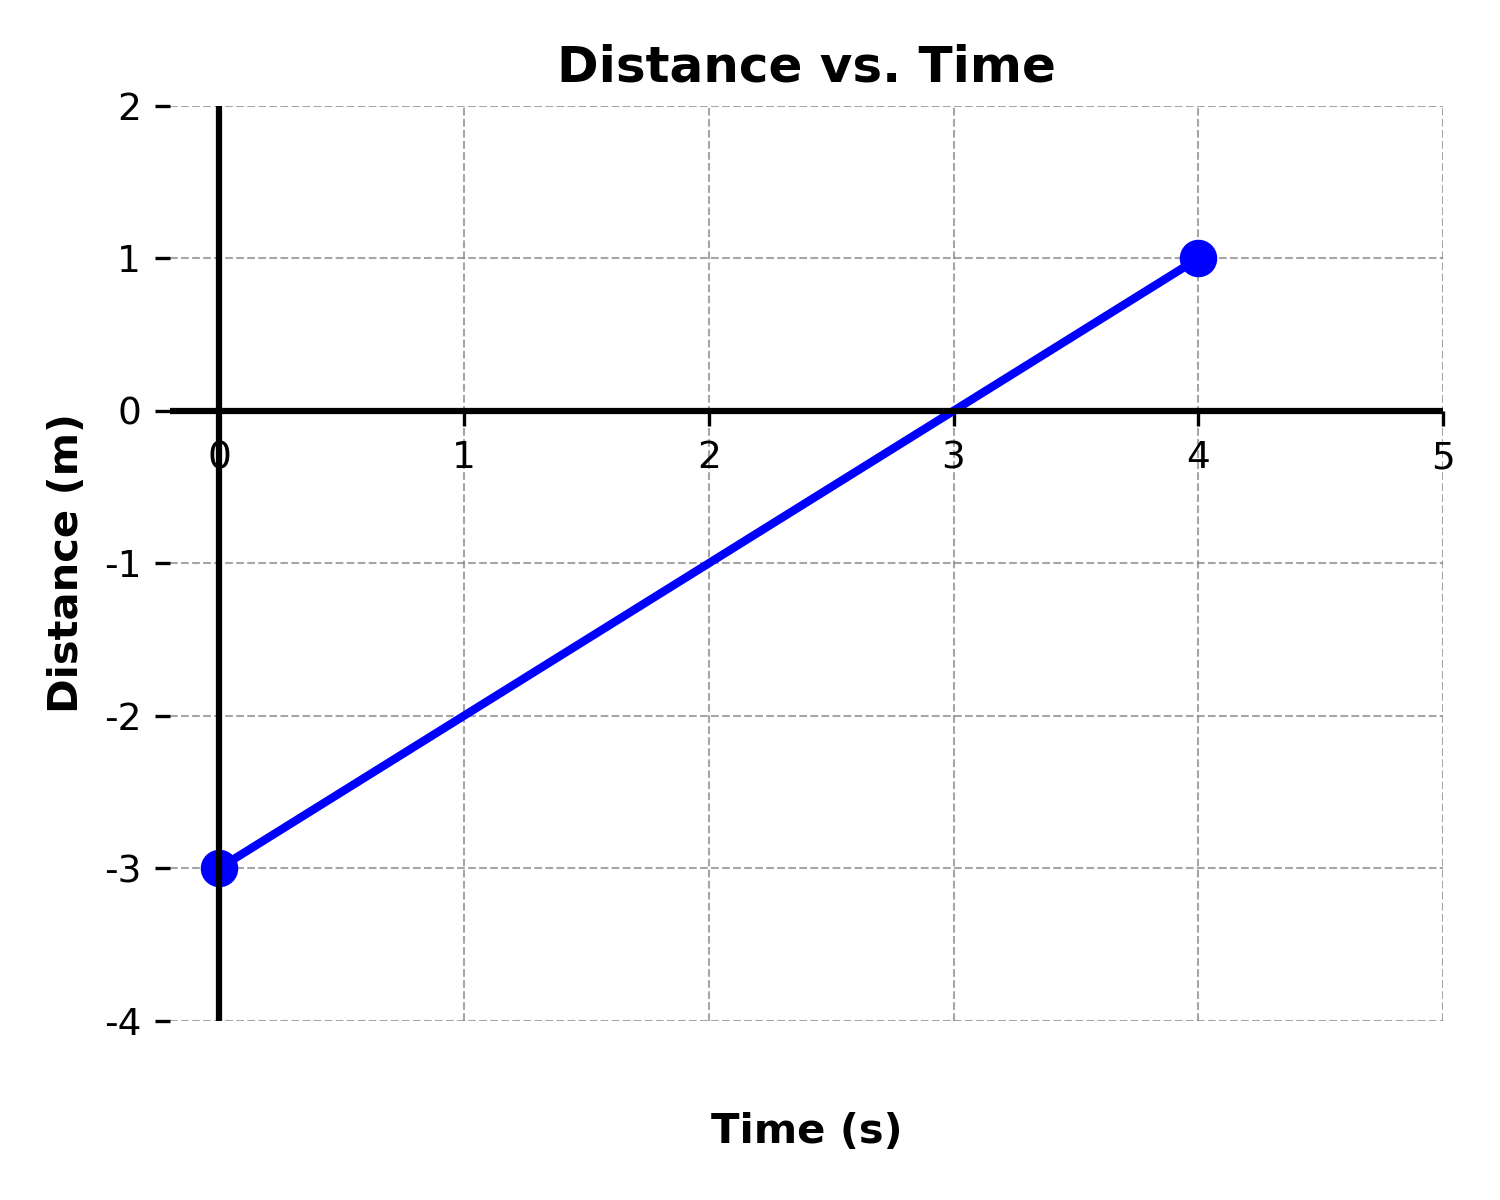
\includegraphics[width=0.6\textwidth]{B_problem_4.png}


\vspace{2cm}  % Add space for students to work
\item Calculate the rate of change from the table below:

\begin{tabular}{|c|c|}
\hline
Time (s) & Distance (m) \\
\hline
0 & -0.3 \\
1 & -1.1 \\
3 & 1.0 \\
5 & 0.4 \\
\hline
\end{tabular}

\vspace{2cm}
\item Calculate the rate of change from the table below:

\begin{tabular}{|c|c|}
\hline
Time (s) & Distance (m) \\
\hline
0 & -0.8 \\
1 & -0.8 \\
2 & -1.5 \\
4 & 1.3 \\
\hline
\end{tabular}

\vspace{2cm}
\item Calculate the rate of change from the table below:

\begin{tabular}{|c|c|}
\hline
Time (s) & Distance (m) \\
\hline
0 & 0.5 \\
1 & -1.0 \\
2 & 0.9 \\
3 & -1.3 \\
\hline
\end{tabular}

\vspace{2cm}
\item Calculate the rate of change from the table below:

\begin{tabular}{|c|c|}
\hline
Time (s) & Distance (m) \\
\hline
0 & 1.8 \\
2 & -1.6 \\
3 & -1.3 \\
5 & -1.9 \\
\hline
\end{tabular}

\vspace{2cm}
\newpage\item An elevator starts at floor 1. After 2 seconds, it is at floor -2. Calculate the rate of change.

\vspace{7cm}
\newpage\item An elevator starts at floor 2. After 2 seconds, it is at floor 0. Calculate the rate of change.

\vspace{7cm}
\end{enumerate}
\newpage
\section*{Answer Key}
\begin{enumerate}
\item The rate of change is $\frac{\Delta y}{\Delta x} = \frac{2--2}{5-0} = 0.8~\text{units/s}$.

\item The rate of change is $\frac{\Delta y}{\Delta x} = \frac{3--2}{5-0} = 1.0~\text{units/s}$.

\item The rate of change is $\frac{\Delta y}{\Delta x} = \frac{-1-2}{3-0} = -1.0~\text{units/s}$.

\item The rate of change is $\frac{\Delta y}{\Delta x} = \frac{1--3}{4-0} = 1.0~\text{units/s}$.

\item The rate of change is $\frac{\Delta y}{\Delta x} = \frac{0.4--0.3}{5-0} = 0.14~\text{units/s}$.

\item The rate of change is $\frac{\Delta y}{\Delta x} = \frac{1.3--0.8}{4-0} = 0.53~\text{units/s}$.

\item The rate of change is $\frac{\Delta y}{\Delta x} = \frac{-1.3-0.5}{3-0} = -0.6~\text{units/s}$.

\item The rate of change is $\frac{\Delta y}{\Delta x} = \frac{-1.9-1.8}{5-0} = -0.74~\text{units/s}$.

\item The rate of change is $\frac{\Delta y}{\Delta x} = \frac{-2-1}{2} = -1.5~\text{floors/s}$.

\item The rate of change is $\frac{\Delta y}{\Delta x} = \frac{0-2}{2} = -1.0~\text{floors/s}$.

\end{enumerate}
\end{document}